\section{Shared batched counter}
\label{ivl-sec:adder}

We now show an example where IVL is inherently less costly than linearizability.
In Section~\ref{ivl-ssec:ivl-adder} we present an IVL batched counter, and show that the {\sc update} operation
has step complexity $O(1)$. The algorithm uses single-writer-multi-reader(SWMR) registers.
In Section~\ref{ivl-ssec:lower-bound} we prove that all linearizable implementations
of a batched counter using SWMR registers have step complexity $\Omega(n)$ for the {\sc update} operation.
This is in contrast with standard (non-batched) counters, which can be implemented with
a constant update time. Intuitively, the difference is that in a standard counter,
all intermediate values ``occur'' in an execution (provided that return values are
all integers and increments all add one),  and so all values allowed by IVL are also
allowed by linearizability.

\subsection{IVL batched counter}
\label{ivl-ssec:ivl-adder}

We consider a \emph{batched counter} object, which supports the operations {\sc update}($v$) where $v \geq 0$, and {\sc read}().
The sequential specification for this object is simple: a {\sc read} operation returns the sum of all values passed to {\sc update}
operations that precede it, and $0$ if no {\sc update} operations were invoked. The {\sc update} operation returns nothing. When the
object is shared, we denote an invocation of {\sc update} by process $i$ as {\sc update}$_i$. We denote the sequential specification
of the batched counter by ${\mathcal H}$.

\begin{algorithm}
    \begin{algorithmic}[1]
        % \begin{multicols}{2}

        \State shared array $v[1 \dots n]$
        \Procedure{update$_i$}{$v$}
        \State $v[i] \gets v[i] + v$
        \EndProcedure

        % \columnbreak

        \Procedure{read}{}
        \State $\mathit{sum} \gets 0$
        \For{$i : 1 \leq i \leq n$}
        \State $\mathit{sum} \gets \mathit{sum} + v[i]$
        \EndFor
        \State \textbf{return} $\mathit{sum}$
        \EndProcedure
    % \end{multicols}
    \end{algorithmic}
    \caption{Algorithm for process $p_i$, implementing an IVL batched counter.}
    \label{ivl-alg:ivl-adder}
\end{algorithm}

Algorithm~\ref{ivl-alg:ivl-adder} presents an IVL implementation for a batched counter
with $n$ processes using an array $v$ of $n$ SWMR registers.
The implementation is a trivial parallelization: an {\sc update} operation increments
the process's local
register while a {\sc read} scans all registers and returns their sum. This
implementation is not linearizable because the reader may see a later {\sc update}
and miss an earlier one, as illustrated in Figure~\ref{ivl-img:adderIVL}.
We now prove the following lemma:
\begin{lemma}
    Algorithm~\ref{ivl-alg:ivl-adder} is an IVL implementation of a batched counter.
    \label{ivl-lmma:ivl-adder}
\end{lemma}
\begin{proof}
    Let $H$ be a well-formed history of an execution $\sigma$ of Algorithm~\ref{ivl-alg:ivl-adder}.
    We first complete $H$ be adding appropriate responses to all {\sc update} operations, and removing all pending {\sc read} operations, we denote
    this completed history as $H'$.

    Let $H_1$ be a linearization of $H'^?$ given by ordering {\sc update} operations by their
    return steps, and ordering {\sc read} operations after all preceding operations in $H'^?$, and before concurrent ones. Operations
    with the same order are ordered arbitrarily.
    Let $H_2$ be a linearization of $H'^?$ given by ordering {\sc update} operations by their
    invocations, and ordering {\sc read} operations operations before all operations that precede them in $H'^?$, and after concurrent ones. Operations
    with the same order are ordered arbitrarily.
    Let $\sigma_i$ for $i=1,2$ be a sequential execution of a batched counter with history $\tau_\mathcal{H}(H_i)$.

    By construction, $H_1$ and $H_2$ are linearizations of $H'^?$. Let $R$ be some {\sc read} operation that completes
    in $H$. Let $v[1 \dots n]$ be the array as read by $R$ in $\sigma$, $v_1[1 \dots n]$ as read by $R$ in $\sigma_1$
    and $v_2[1 \dots n]$ as read by $R$ in $\sigma_2$. To show that
    $\text{ret}(R, \tau_\mathcal{H}(H_1)) \leq \text{ret}(R, H) \leq \text{ret}(R, \tau_\mathcal{H}(H_2))$,
    we show that $v_1[j] \leq v[j] \leq v_2[j]$ for every index $1 \leq j \leq n$.

    For some index $j$, only $p_j$ can increment $v[j]$. By the construction of $H_1$, all {\sc update} operations
    that precede $R$ in $H$ also precede it in $H_1$. Therefore $v_1[j] \leq v[j]$. Assume by contradiction that $v[j] > v_2[j]$.
    Consider all concurrent {\sc update} operations to $R$. After all concurrent {\sc update} operations end, the value
    of index $j$ is $v' \geq v[j] > v_2[j]$. However, by construction, $R$ is ordered after all concurrent {\sc update}
    operations in $H_2$, therefore $v' \leq v_2[j]$. This is a contradiction, and therefore $v[j] \leq v_2[j]$.

    As all entries in the array are non-negative, it follows that $\sum_{j=1}^n v_1[j] \leq \sum_{j=1}^n v[j] \leq \sum_{j=1}^n v_2[j]$, and
    therefore $\text{ret}(R, \tau_\mathcal{H}(H_1)) \leq \text{ret}(R, H) \leq \text{ret}(R, \tau_\mathcal{H}(H_2))$.
\end{proof}

Figure~\ref{ivl-img:adderIVL} shows a possible concurrent execution of Algorithm~\ref{ivl-alg:ivl-adder}.
This algorithm can efficiently implement a distributed or NUMA-friendly counter, as processes
only \inred{update} their local registers thereby lowering the cost of incrementing the counter. This is of
great importance, as memory latencies are often the main bottleneck in shared object emulations~\cite{mahapatra1999processor}.
As there are no waits in
either {\sc update} or {\sc read}, it follows that the algorithm is wait-free. Furthermore, the {\sc read} step complexity
is $O(n)$, and the {\sc update} step complexity is $O(1)$. Thus, we have shown the following theorem:
\begin{theorem}
    There exists a bounded wait-free IVL implementation of a batched counter using only SWMR registers, such that the step complexity of {\sc update} is $O(1)$
    and the step complexity of {\sc read} is $O(n)$.
\end{theorem}

\begin{figure}[b]
    \centering
    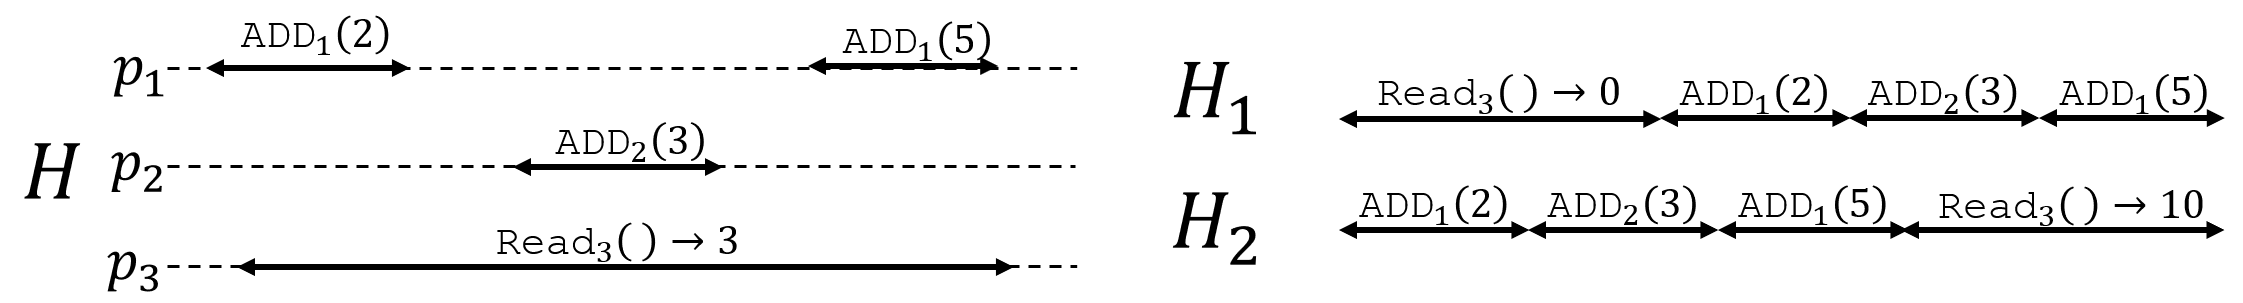
\includegraphics[width=0.7\textwidth]{images/adderIVL.png}
    \caption{A possible concurrent history of the IVL batched counter: $p_1$ and
    $p_2$ update their local registers, while $p_3$ reads. $p_3$ returns an intermediate
    value between the counter's state when it starts, which is $0$, and the counter's state when it completes, which is $10$.}
    \label{ivl-img:adderIVL}
\end{figure}
